\documentclass[a4paper, english, twoside, 12pt]{article}
\usepackage[margin=2cm]{geometry}
\usepackage{amsmath}
\usepackage[utf8]{inputenc}    %nice copy and pasting
\usepackage[T1]{fontenc}       %makes text copy-and-pastable
%\usepackage{natbib}            %for bibliography stuff
\usepackage{graphicx}          %for images
\usepackage{epstopdf} 			%To import unsw emblem and stuff
\usepackage[acronym, nomain]{glossaries}

\makeglossaries
\newacronym{set}{SET}{Single Electron Transistor}
\newacronym{cqc2t}{CQC2T}{Centre for Quantum Computation and Communication Technology}
\newacronym{pcie}{PCIe}{Peripheral Component Interconnect Express}
\newacronym{dma}{DMA}{Direct Memory Access}
\newacronym{adc}{ADC}{Analogue to Digital Converter}
\newacronym{fpga}{FPGA}{Field-Programmable Gate Array}

%\DeclareGraphicsExtensions{.eps}

\usepackage{wrapfig}           %for figures
%\usepackage[export]{adjustbox} %for putting boxes around figures
\usepackage{url}               %allow pretty formating of URLs \url{www.example.com}
\usepackage{booktabs}          % good tables package
\usepackage{multirow}          %merging table cells
\usepackage{varioref}          %for doing "table x on page y" with \vref{tab:label}
\usepackage{caption}           %to use minipage for inserting figures
\usepackage{float}             %for H figure and table placements Here.
\usepackage{pdfpages}          %To include pdfs
\usepackage[nottoc, notlot, notlof, numbib]{tocbibind} %Number the references section
\usepackage[title, titletoc, header]{appendix}
\usepackage{tikz}
%\usepackage{array}
%\newcolumntype{L}[1]{>{\raggedright\let\newline\\\arraybackslash\hspace{0pt}}m{#1}}
%\newcolumntype{C}[1]{>{\centering\let\newline\\\arraybackslash\hspace{0pt}}m{#1}}
%\newcolumntype{R}[1]{>{\raggedleft\let\newline\\\arraybackslash\hspace{0pt}}m{#1}}

\raggedbottom


%these 3 lines automatically render opening double quotes the right way around
%(They normally appear backwards)
\usepackage [english]{babel}
\usepackage [autostyle, english = american]{csquotes}
\MakeOuterQuote{"}
\usepackage{rotating}
\usepackage{subcaption}

%\usepackage[colorinlistoftodos]{todonotes}%to do notes
\usepackage[disable]{todonotes} %Uncomment for the final version


\graphicspath{{./img/}}

\setcounter{tocdepth}{2}% remove subsubsections from table of contents
   
%This package must go last, or it won't work
%With this package, you can click on cross references, URLs and page numbers, and you'll be taken there.
\usepackage[hidelinks,%clickable cross references and URLs, without visable formatting
            pdftex,%pdf meta data
            %pdfauthor={},%pdf meta data
            pdftitle={z3421023 Thesis A Report},%pdf meta data
            ]{hyperref}
\begin{document}

\pagenumbering{roman}
%\includepdf{./src/cover_sheet.pdf}
\pagenumbering{arabic}

%  Include the cover page
\thispagestyle{empty}
\begin{center}
	\centering
\includegraphics[width=0.8\textwidth]{Arms-vl}\\
	[0.5cm]
\textbf{\large SCHOOL OF ELECTRICAL ENGINEERING\\
AND TELECOMMUNICATION}\\[2cm]
{\addtolength{\baselineskip}{0.5cm}
\textbf{\Huge
Ultra-High Fidelity Spin Qubit Initialization with Digital Feedback} \\[0.5cm]
}
{\Large by}\\[0.5cm]
\textit{\huge
Mark Johnson} \\[1.5cm]
{\Large
Interim Thesis A (ELEC4120) Report\\[2ex]
\vfill
Submitted: \today\hfill
Student ID: z3421023\\[-1.0ex]
Supervisor: Andrea Morello\hfill
Topic ID: AM5\\
\vspace*{-1cm}
}
\end{center}
\pagebreak


\listoftodos

\pagebreak

% Disable first glossary references in list of figures, or table of contents
\glsunsetall
\tableofcontents
\listoffigures
% Resets glossary references
\glsresetall
\pagebreak

\section{Abstract}
Quantum computers present a new paradigm for solving various tasks. A general purpose quantum computer has been proved to exceed a classical computer in certain applications, such as sorting a database, and is inherently better at modelling quantum effects and performing simulations, which has large implications for the drug industry and chemical engineering broadly. This report aims to introduce the concept of a quantum computer, and current attempts at creating and controlling qubits, quantum bits of information. The body of work in this thesis is geared towards improving qubit state initialization fidelity, which would make all further experiments for efficient and cost effective. The prime way of improving initialization is to incorporate a feedback loop that will self-correct for any potential error before proceeding with any further operations on the qubit. Digital systems have been used to great effect in closing the loop, and this is the approach taken through this report.
\pagebreak
\section{Introduction}
Modern computing devices are becoming ever smaller, and to remain functional they must be engineered to combat the encroaching quantum effects at these scales, with increasing difficulty. Intel's current process incorporates a 14nm FET channel, as such the design of these FETs has been greatly changed to eliminate quantum effects. \cite{intel_process} In the near future, Intel will continue moving to a 10nm process which is presenting with further challenges. \cite{intel_future}

The trend in transistor miniaturisation has been dubbed "Moore's Law", following a prediction made by Gordon Moore, co-founder of Intel, in 1965. \cite{moore1965cramming}

\begin{quotation}
	"The complexity for minimum component costs has increased at a rate of roughly a factor of
	 two per year ... Certainly over the short term this rate
	can be expected to continue, if not to increase." 
\end{quotation}
 Despite the remarkable accuracy of this prediction, many believe \cite{end_of_Moore_1, end_of_Moore_2} the inevitable breakdown of this rule will take place as the physical limitations of creating such devices exponentially increases the start-up cost of manufacturing, as well as the cost of research and development.

However, this brick-wall has sparked research into alternative forms of computation. One such example, is a general purpose quantum computer. A quantum computer is unlike any classical computer, in the sense that its principles of operation are entirely based on quantum mechanics, as opposed to the classical electronics which modern computers are designed from. The difference between these paradigms cannot be understated, and one is not simply a replacement for the other. Despite the lack of a working quantum computer at this point in time, many researchers have spent time designing certain algorithms and processes that would run on such a machine, and analysing the benefits of the architecture compared to the classical computer. One such example is Grover's algorithm \cite{grover1996fast}, which is a method to sort databases which has a worst-case execution time of $\mathcal{O}(\sqrt{n})$, a remarkable improvement over the theoretical limit of any classical comparison based algorithm, $\mathcal{O}(n \log{n})$.


\todo[inline]{Introduce the work I'm doing, in particular. Describe structure of document}

\begin{figure}[htbp!]
	\centering
	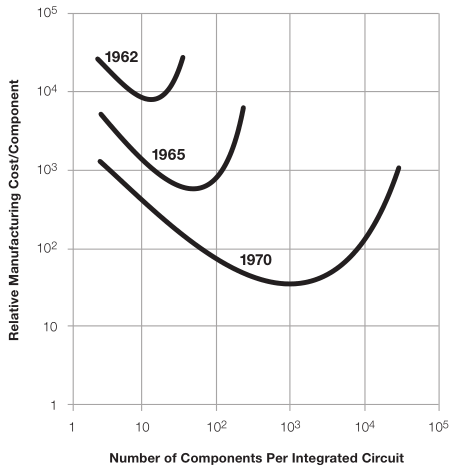
\includegraphics[width=0.8\textwidth]{moores_law}
	\caption{Gordon Moore's Prediction on Component Cost - Moore's Law}
	\label{fig::moores_law}
\end{figure}

\pagebreak
\section{Literature Review}
\subsection{State of the Art}
% Review all of the current experimental evidence pertaining to my area of research
\todo[inline]{Talk quantum electron spin, projective measurement vs non-projective measurement (bloch sphere), about technology behind SETs}
\cite{nuclear_spin_readout}
\subsection{Devices}
\subsubsection{PCIe Digitizer Card}
\todo[inline]{Talking points of the Digitizer solution, DMA, etc. etc.}
%\subsubsection{FPGA/$\mu$Controller and ADC}
\todo[inline]{Talking points of the external FPGA and ADC solution, mention some particular examples of ADCs etc.}
\subsubsection{XMC}
\todo[inline]{Talking points of the integrated XMC solution, pre-built FPGA, ADCs and possibly with Auto-DMA}

\pagebreak
\section{Experimental Design}
With new devices constantly being designed and fabricated, new avenues being probed, the structure of experiments can become convoluted. The needless post-processing of all acquired data to top it all of is \todo[inline]{gargghh}


The apparatus I am applying my work to is by no means comprehensive, but it serves as a reference point in a proven device. To accomplish this body of work with this particular device would 


Figure \ref{fig::set_layout} shows the physical device that will be similar to one I will be testing my solution on. This devices has various control points, such as the top gate to induce a layer of electrons on the boundary, the left and right barriers to remove this layer, forming tunnel junctions to the island, and finally the plunger to control the gate, as in a MOSFET.

\begin{figure}[htbp!]
	\centering
	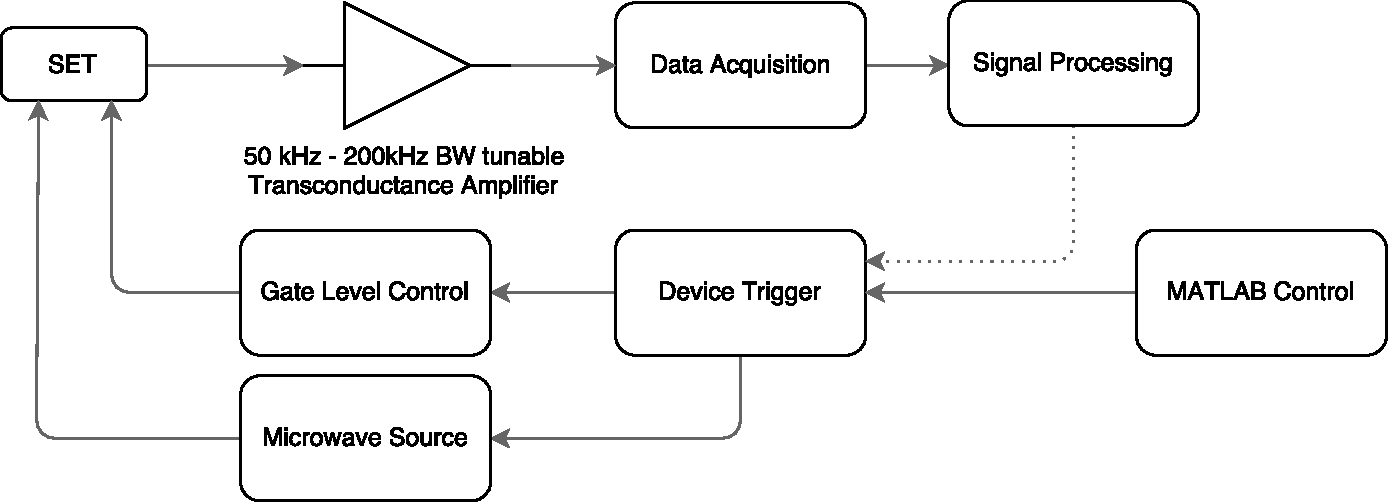
\includegraphics[width=\textwidth]{thesis_experiment.pdf}
	\caption{Block diagram of experiment}
	\label{fig::thesis_experiment}
\end{figure}

\begin{figure}[htbp!]
	\centering
	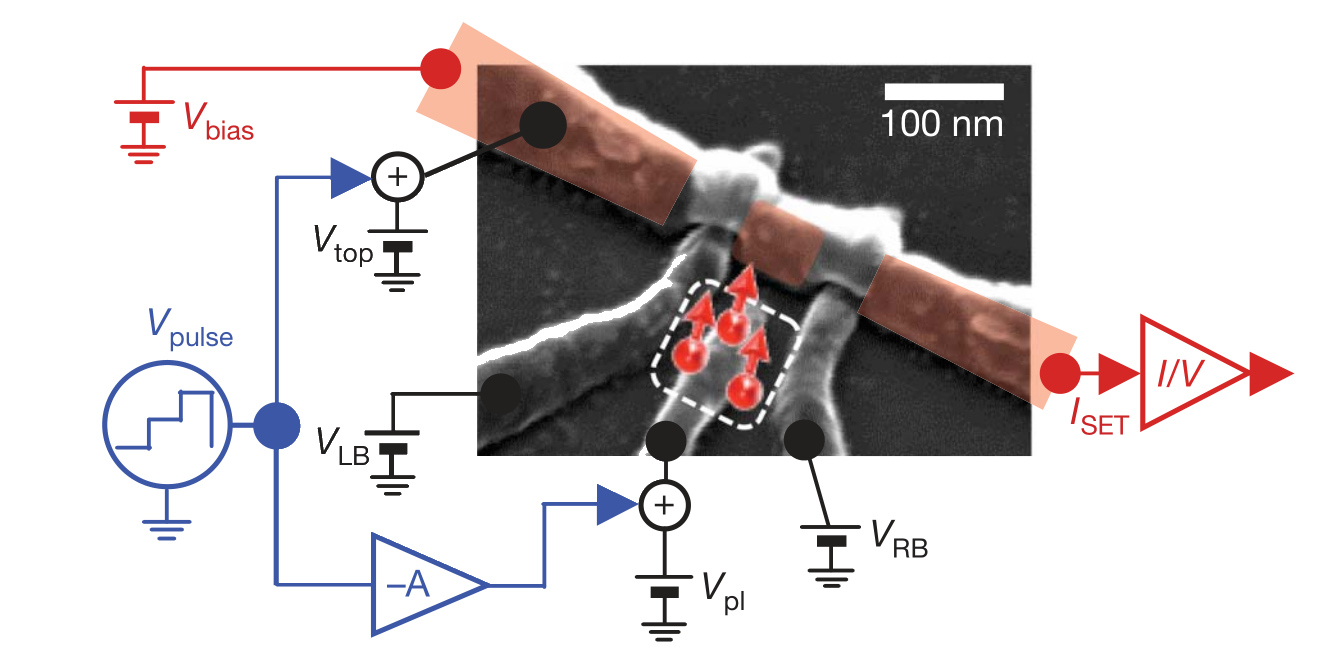
\includegraphics[width=\textwidth]{set_layout}
	\caption{The layout of an SET}
	\label{fig::set_layout}
\end{figure}

\begin{figure}[htbp!]
	\centering
	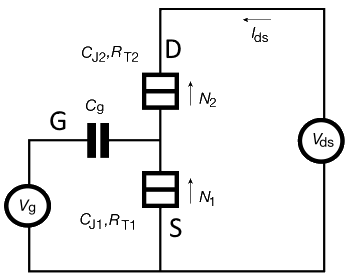
\includegraphics[width=0.6\textwidth]{set_circuit}
	\caption{Equivalent electrical circuit of an SET}
	\label{fig::set_circuit}
\end{figure}

\begin{figure}[htbp!]
	\centering
	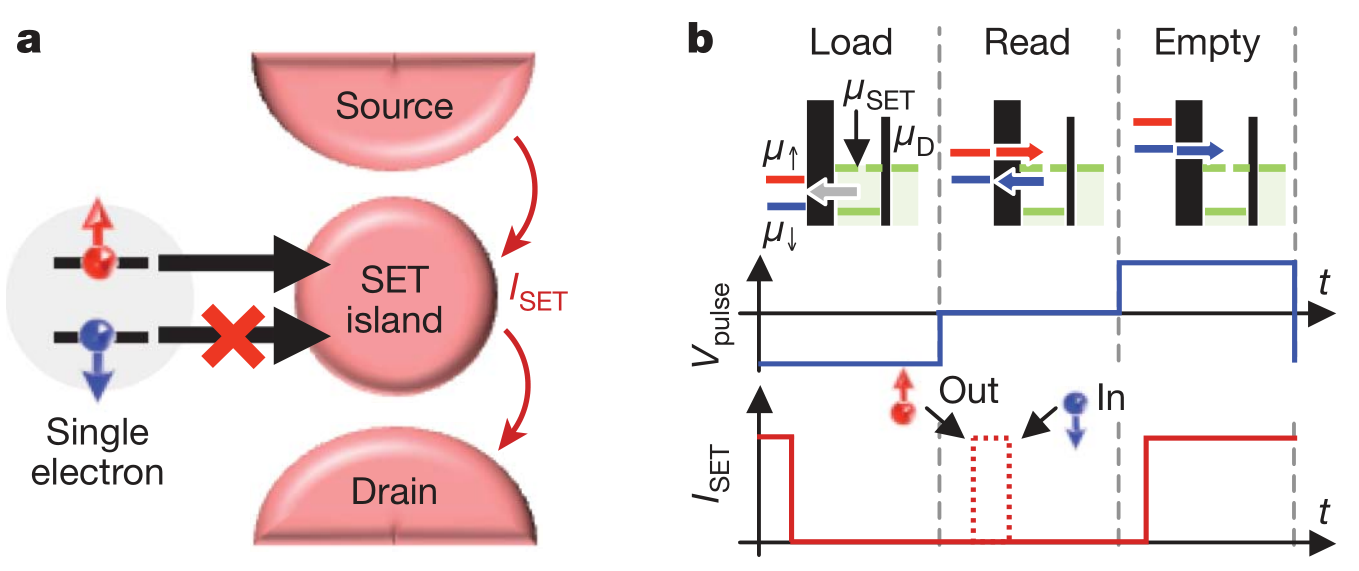
\includegraphics[width=\textwidth]{set_loading}
	\caption{The initialisation procedure of an SET}
	\label{fig::set_loading}
\end{figure}
\pagebreak
\section{Prospective Plan}
\subsection{Proposed Timeline}
%\todo[inline]{A Gantt chart, perhaps with critical tasks highlighted, to be detailed below}
Figure \ref{fig::gantt_chart} shows my proposed timeline to complete my thesis work. Most work is to be completed during the first semester of next year, though I have organised to get as much research complete over the summer break so I can use my time more appropriately during semester. The red bars show an alternate pathway to a working solution, if the \gls{pcie} digitizer or MATLAB is unable to perform the required task.
\begin{figure}[htbp!]
	\centering
	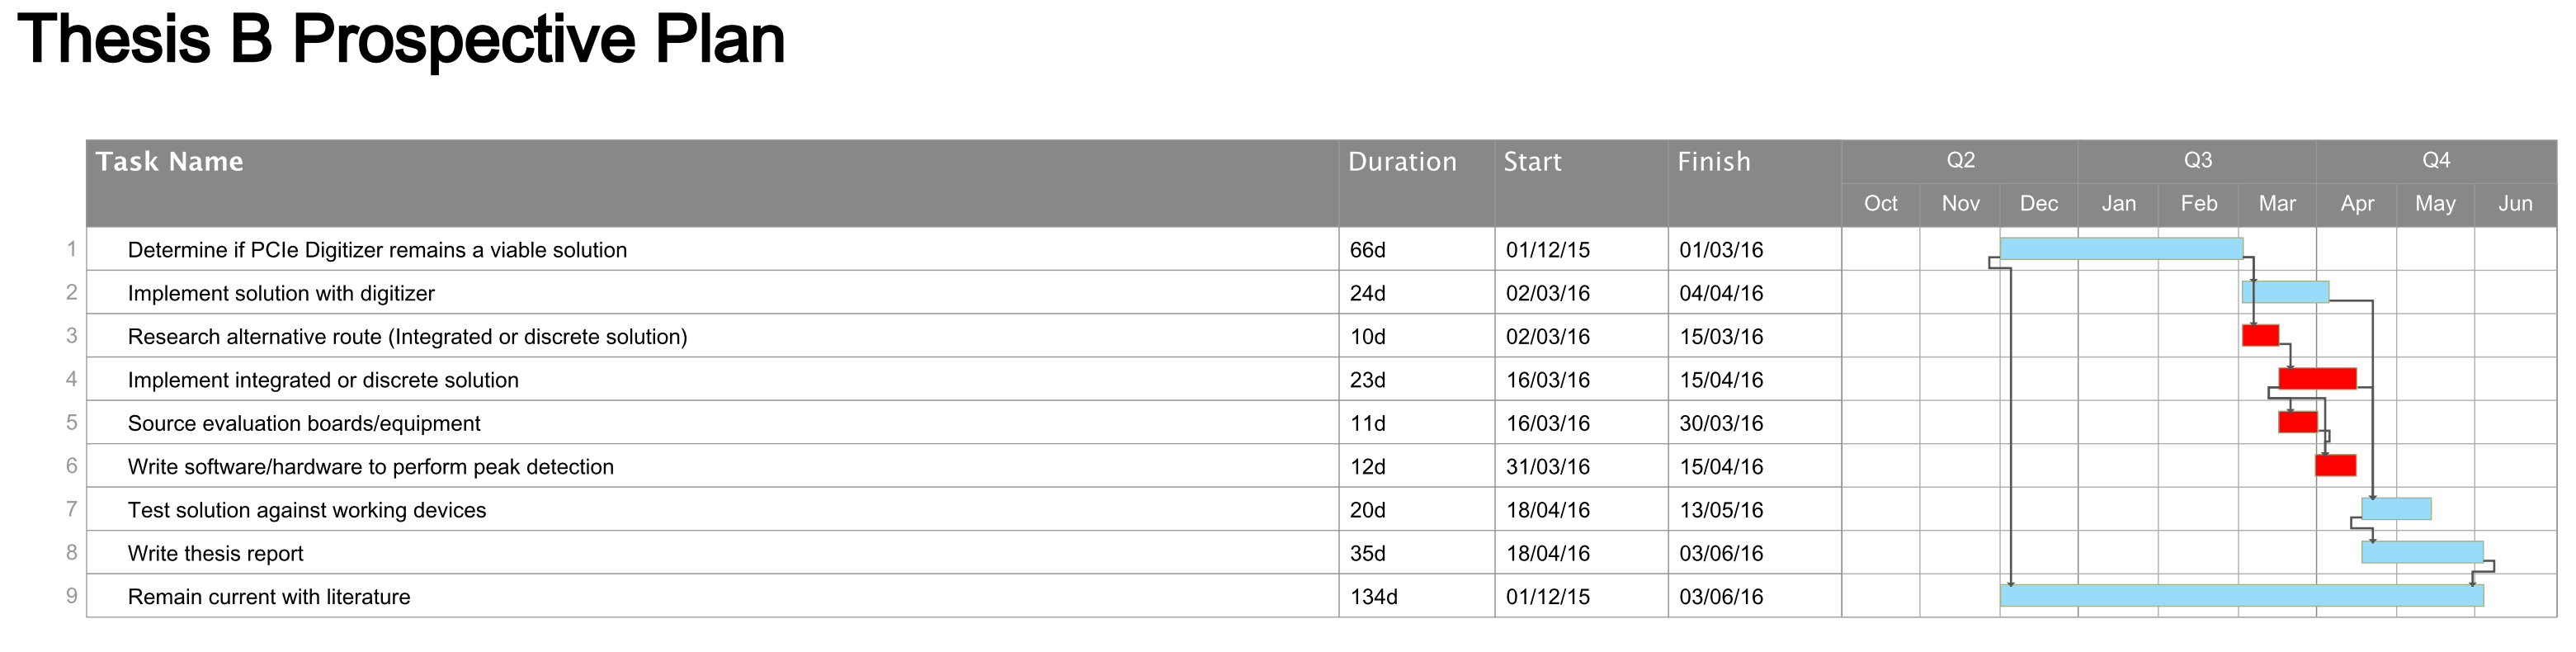
\includegraphics[width=\textwidth, height=0.3\textheight]{gantt_chart}
	\caption{Gantt Chart for Thesis B, beginning December}
	\label{fig::gantt_chart}
\end{figure}

\subsection{Description of Work}

The following lists are the final avenues available in utilizing the \gls{pcie} digitizer and MATLAB solution.
\begin{itemize}
	\item Software Triggering
	\item Continuous \gls{dma}
	\item Manual external triggering
\end{itemize}
By the beginning of semester I will be able to confirm or deny if any of these solutions will work. The software triggering is a feature of the digitizer, where you can call a function directly from MATLAB to cause a \gls{dma} buffer to be filled, until one full acquisition has been achieved. Alternatively, there is the Continuous \gls{dma} which after a single trigger, can supposedly continue to acquire a pre-determined amount of samples, though I'm not sure of the resolution of data access, for example, if I can only process the data in 1 second windows, that isn't useful. The final method should always work, supposing that the machine MATLAB is running on can perform the signal processing in the meantime between acquisitions. Manual external triggering can be achieved from a PulseBlaster Programmable TTL Pulse Generator, a device currently being used as the device trigger in Figure \ref{fig::thesis_experiment} of Section \ref{sec::experiment}. In the event that these solutions do not work, I will proceed with designing and sourcing some evaluation boards for a precision \gls{adc} and a $\mu$controller or FPGA.

Finding the right \gls{adc} is fairly important, as the conditions of the measured signal often change between experiments. The dynamic range should be adjustable, ideally with lower settings of about $\pm 100$mV, and also a sampling rate fairly close to 5 \gls{msps}. It is undesirable to exceed this sample rate, as it would increase the workload for the signal processor.

Once the software or hardware has been implemented, I will characterise the improvement in readout fidelity. At this stage, I will most likely be adjusting the wait time, trying to achieve 99.9\% initialization fidelity. To characterise the device, I will need an electron donor device with an \gls{set} for readout, which are currently being designed and manufactured within \gls{cqc2t}.

Concurrently with this, I can begin writing my thesis B report, initially detailing the design process and all explored avenues in this problem, then once I have tested my solution I will be able to conclude whether it did or didn't work, and why.

%\todo[inline]{Details about what the particulars of work to be done are}

%\todo[inline]{Talk about further options with PCIe digitizer, manual triggering in MATLAB, manual external triggering from an ARB (software controlled), or continuous DMA}
\pagebreak
\section{Conclusion}
%\todo[inline]{Conclude, like normal}
A quantum computer is the ultimate goal of researchers within \gls{cqc2t}, and devices and experiments are continuously being devised to this end. Devices have been composed of an \gls{set} for spin-dependent readout, a must for a spin-based quantum computer, and experiments are constructed at cryogenic temperatures, and spin qubit manipulation is performed with series of microwave pulses. Before you perform operations on a qubit, it needs to start in a well defined state, and current methods rely on pre-selection of data, based on the criterion of having an electron present at the commencement of the operations. This is an inefficient use of time, and this can be improved by incorporating a digital feedback loop that will perform a strong measurement on the electron spin, and signal the continuation of an experiment.

In my literary review, I have covered some of the fundamental concepts governing the devices being used currently in this research, as well as some other research into the use of digital feedback in quantum systems.
The experimental design explored how the devices were being used together, and where the solution of this thesis will be place in the larger system. It also details some proposed solutions to the lack of digital feedback.
Finally, the prospective plan lists various tasks that are to be completed, from a high-level perspective by the completion of Thesis B.
\pagebreak
\bibliographystyle{ieeetr}	%IEEE style referencing
\bibliography{./src/references}
\pagebreak
\begin{appendices} 
	\section{Glossary}
	\printglossaries
	\section{Risk Assessment}
	Attached below.
	\includepdf[landscape=true,pages={1-3}]{./src/risk_management.pdf}	
	\section{Supplementary Information}
	\paragraph{Big O Notation} describes the limiting behaviour of a function when the argument tends toward infinity.
\label{supp::big_o}
For example, the leading term ($3 x^4$) in the polynomial $p(x) = 3 x^4 + 20 x^2 + 1$, represents the strongest factor that determines the behaviour of the function. As such, we say $p$ has order $\mathcal{O}(n^4)$. Note that we drop any constant multiplier as it doesn't modify the growth or shape of the function.
\end{appendices}
\end{document}
